\documentclass[a4paper,12pt]{exam}
\printanswers % pour imprimer les réponses (corrigé)
%\noprintanswers % Pour ne pas imprimer les réponses (énoncé)
\addpoints % Pour compter les points
% \noaddpoints % pour ne pas compter les points
%\pointsinmargin
%\qformat{\textbf{\thequestion ) } }
%\qformat{\textbf{\thequestion )} (\textit{\thepoints}) \\  }  % Pour définir le style des questions (facultatif)
\usepackage{color} % définit une nouvelle couleur
\shadedsolutions % définit le style des réponses
% \framedsolutions % définit le style des réponses
\definecolor{SolutionColor}{rgb}{0.8,0.9,1} % bleu ciel
\renewcommand{\solutiontitle}{\noindent\textbf{Solution:}\par\noindent} % Définit le titre des solutions




\makeatletter

\def\maketitle{{\centering%
	\par{\huge\textbf{\@title}}%
	\par{\@date}%
	\par}}


\renewcommand{\thesubsection}{\Alph{subsection}.}   

\makeatother

%\lhead{NOM Pr\'enom :}
%\rhead{\textbf{Les r\'eponses doivent \^etre justifi\'ees et r\'edig\'ees}}
\cfoot{\thepage / \pageref{LastPage}}


%\usepackage{../../pas-math}
%\usepackage{../../moncours}


%\usepackage{pas-cours}
%-------------------------------------------------------------------------------
%          -Packages nécessaires pour écrire en Français et en UTF8-
%-------------------------------------------------------------------------------
\usepackage[utf8]{inputenc}
\usepackage[frenchb]{babel}
\usepackage[T1]{fontenc}
\usepackage{lmodern}
\usepackage{textcomp}



%-------------------------------------------------------------------------------

%-------------------------------------------------------------------------------
%                          -Outils de mise en forme-
%-------------------------------------------------------------------------------
\usepackage{hyperref}
\hypersetup{pdfstartview=XYZ}
%\usepackage{enumerate}
\usepackage{graphicx}
\usepackage{multicol}
\usepackage{tabularx}
\usepackage{multirow}


\usepackage{anysize} %%pour pouvoir mettre les marges qu'on veut
%\marginsize{2.5cm}{2.5cm}{2.5cm}{2.5cm}

\usepackage{indentfirst} %%pour que les premier paragraphes soient aussi indentés
\usepackage{verbatim}
\usepackage{enumitem}
\usepackage[usenames,dvipsnames,svgnames,table]{xcolor}

\usepackage{variations}

%-------------------------------------------------------------------------------


%-------------------------------------------------------------------------------
%                  -Nécessaires pour écrire des mathématiques-
%-------------------------------------------------------------------------------
\usepackage{amsfonts}
\usepackage{amssymb}
\usepackage{amsmath}
\usepackage{amsthm}
\usepackage{tikz}
\usepackage{xlop}
%-------------------------------------------------------------------------------



%-------------------------------------------------------------------------------


%-------------------------------------------------------------------------------
%                    - Mise en forme avancée
%-------------------------------------------------------------------------------

\usepackage{ifthen}
\usepackage{ifmtarg}


\newcommand{\ifTrue}[2]{\ifthenelse{\equal{#1}{true}}{#2}{$\qquad \qquad$}}

%-------------------------------------------------------------------------------

%-------------------------------------------------------------------------------
%                     -Mise en forme d'exercices-
%-------------------------------------------------------------------------------
%\newtheoremstyle{exostyle}
%{\topsep}% espace avant
%{\topsep}% espace apres
%{}% Police utilisee par le style de thm
%{}% Indentation (vide = aucune, \parindent = indentation paragraphe)
%{\bfseries}% Police du titre de thm
%{.}% Signe de ponctuation apres le titre du thm
%{ }% Espace apres le titre du thm (\newline = linebreak)
%{\thmname{#1}\thmnumber{ #2}\thmnote{. \normalfont{\textit{#3}}}}% composants du titre du thm : \thmname = nom du thm, \thmnumber = numéro du thm, \thmnote = sous-titre du thm

%\theoremstyle{exostyle}
%\newtheorem{exercice}{Exercice}
%
%\newenvironment{questions}{
%\begin{enumerate}[\hspace{12pt}\bfseries\itshape a.]}{\end{enumerate}
%} %mettre un 1 à la place du a si on veut des numéros au lieu de lettres pour les questions 
%-------------------------------------------------------------------------------

%-------------------------------------------------------------------------------
%                    - Mise en forme de tableaux -
%-------------------------------------------------------------------------------

\renewcommand{\arraystretch}{1.7}

\setlength{\tabcolsep}{1.2cm}

%-------------------------------------------------------------------------------



%-------------------------------------------------------------------------------
%                    - Racourcis d'écriture -
%-------------------------------------------------------------------------------

% Angles orientés (couples de vecteurs)
\newcommand{\aopp}[2]{(\vec{#1}, \vec{#2})} %Les deuc vecteurs sont positifs
\newcommand{\aopn}[2]{(\vec{#1}, -\vec{#2})} %Le second vecteur est négatif
\newcommand{\aonp}[2]{(-\vec{#1}, \vec{#2})} %Le premier vecteur est négatif
\newcommand{\aonn}[2]{(-\vec{#1}, -\vec{#2})} %Les deux vecteurs sont négatifs

%Ensembles mathématiques
\newcommand{\naturels}{\mathbb{N}} %Nombres naturels
\newcommand{\relatifs}{\mathbb{Z}} %Nombres relatifs
\newcommand{\rationnels}{\mathbb{Q}} %Nombres rationnels
\newcommand{\reels}{\mathbb{R}} %Nombres réels
\newcommand{\complexes}{\mathbb{C}} %Nombres complexes


%Intégration des parenthèses aux cosinus
\newcommand{\cosP}[1]{\cos\left(#1\right)}
\newcommand{\sinP}[1]{\sin\left(#1\right)}


%Probas stats
\newcommand{\stat}{statistique}
\newcommand{\stats}{statistiques}
%-------------------------------------------------------------------------------

%-------------------------------------------------------------------------------
%                    - Mise en page -
%-------------------------------------------------------------------------------

\newcommand{\twoCol}[1]{\begin{multicols}{2}#1\end{multicols}}


\setenumerate[1]{font=\bfseries,label=\textit{\alph*})}
\setenumerate[2]{font=\bfseries,label=\arabic*)}


%-------------------------------------------------------------------------------
%                    - Elements cours -
%-------------------------------------------------------------------------------





%\usepackage{fullpage}
\author{\ }

%Ex 2 nouvelle calédonie 2018 ex 2 (8 pts)
%Ex 1 metropole remplacement 2018 ex 1 (6 pts)

\begin{document}
%	\usepackage{fancyhdr}
%	
%	\pagestyle{fancy}
%	\fancyhf{}
	%\rhead{Share\LaTeX}

	%\maketitle
	
	\begin{center}
	%\centering
	
	{\scshape\LARGE \textbf{BACCALAUR\'EAT TECHNOLOGIQUE} \par}
	\vspace{1cm}
	{\scshape\Large \textbf{SESSION 2018}\par}
	\vspace{1.5cm}
	

	\begin{large}
		\begin{tabular}{|@{\ }c@{\ }|@{\ }c@{\ }|}
		\hline
		%\ & \ \\
		\'Epreuve : \textbf{MATH\'EMATIQUES} & Série : \textbf{Sciences et Technologies de}  \\ 
		\textit{\'Epreuve blanche}&  \textbf{la Santé et du Social (ST2S)} \\ \hline
		\ & \ \\
		Durée de l'épreuve : \textbf{2 heures} & Coefficient : \textbf{3} \\ 
		\ & \ \\
		\hline
	\end{tabular}
	\end{large}
		
	\vspace{1cm}
	{\large\bfseries \'EPREUVE DU MERCREDI 26 AVRIL 2018}
	
	\vspace{1cm}
	{\itshape L'usage d'une calculatrice autorisé selon la réglementation en vigueur\par}
	%\vfill
	\vspace{1.5cm}
	{\bfseries Ce sujet comporte \pageref{LastPage} pages numérotées de 1/\pageref{LastPage} à \pageref{LastPage}/\pageref{LastPage} }
	
%	\vspace{0.5cm}
%	{\bfseries Ce sujet comporte x annexes situés pages \pageref{annexe} /\pageref{LastPage} à \pageref{LastPage}/\pageref{LastPage} à remettre avec la copie.}
	
	\vspace{0.5cm}
	{\bfseries\itshape Le candidat doit s'assurer que le sujet distribué est complet. }
	
	\vfill	
	
	\fbox{
		\begin{minipage}{0.9\textwidth}
			\large
			Il  est  rappelé  que  la  qualité  de  la  rédaction,  la  clarté  et  la  précision  des  raisonnements entreront pour une part importante dans l'appréciation des copies. 
			
			Cependant, le candidat est invité à faire figurer sur la copie toute trace de recherche, même incomplète ou infructueuse, qu'il aura développée. 
		\end{minipage}
	}
	
	\vfill

% Bottom of the page
	%{\large \today\par}
\end{center}
\newpage

\ 
\ 
\\

\newpage

\section{(6 points)}\label{ex:secu}

La loi de financement de la Sécurité sociale comprend un objectif national de dépenses d'assurance maladie, qui est voté chaque année par le Parlement.

Le montant des dépenses d'assurance maladie a été évalué pour l'année 2016 à \num{185.2} milliards d'euros. Le parlement a voté une croissance de ces dépenses de \num{2.1} \% pour l'année 2017.



\begin{questions}
	\question Montrer que le montant des dépenses  d'assurance maladie voté pour l'année 2017 est de \num{189.1} milliards d'euros \emph{(à cent millions près)}.
	
	\begin{solution}
		Le coefficient multiplicateur correspondant à une augmentation de \num{2.1} \%, est \num{1.021}.
		
		\begin{equation*}
			\num{185.2} \times \num{1.021} \approx \num{189.08}
		\end{equation*}
		
		Le montant des dépenses  d'assurance maladie voté pour l'année 2017 est donc bien de \num{189.1} milliards d'euros.
	\end{solution}
	
	
	
\end{questions}



Pour estimer les montants des années suivantes, on suppose que le Parlement votera chaque année une augmentation de \num{2.1} \% de ces dépenses.

On modélise à l'aide d'une suite $(v_n)$ le montant, en milliards d'euros des dépenses d'assurance maladie voté chaque année. On note $v_0$ le montant voté pour l'année 2016 et $v_n$ le montant voté pour l'année (2016 + $n$), où $n$ est un entier positif ou nul. On a ainsi $v_0 = \num{185.2}$.


 On veut utiliser la feuille de calcul automatisé ci-dessous afin d'obtenir les valeurs successives de la suite $(v_n)$.
 
 \begin{center}
 	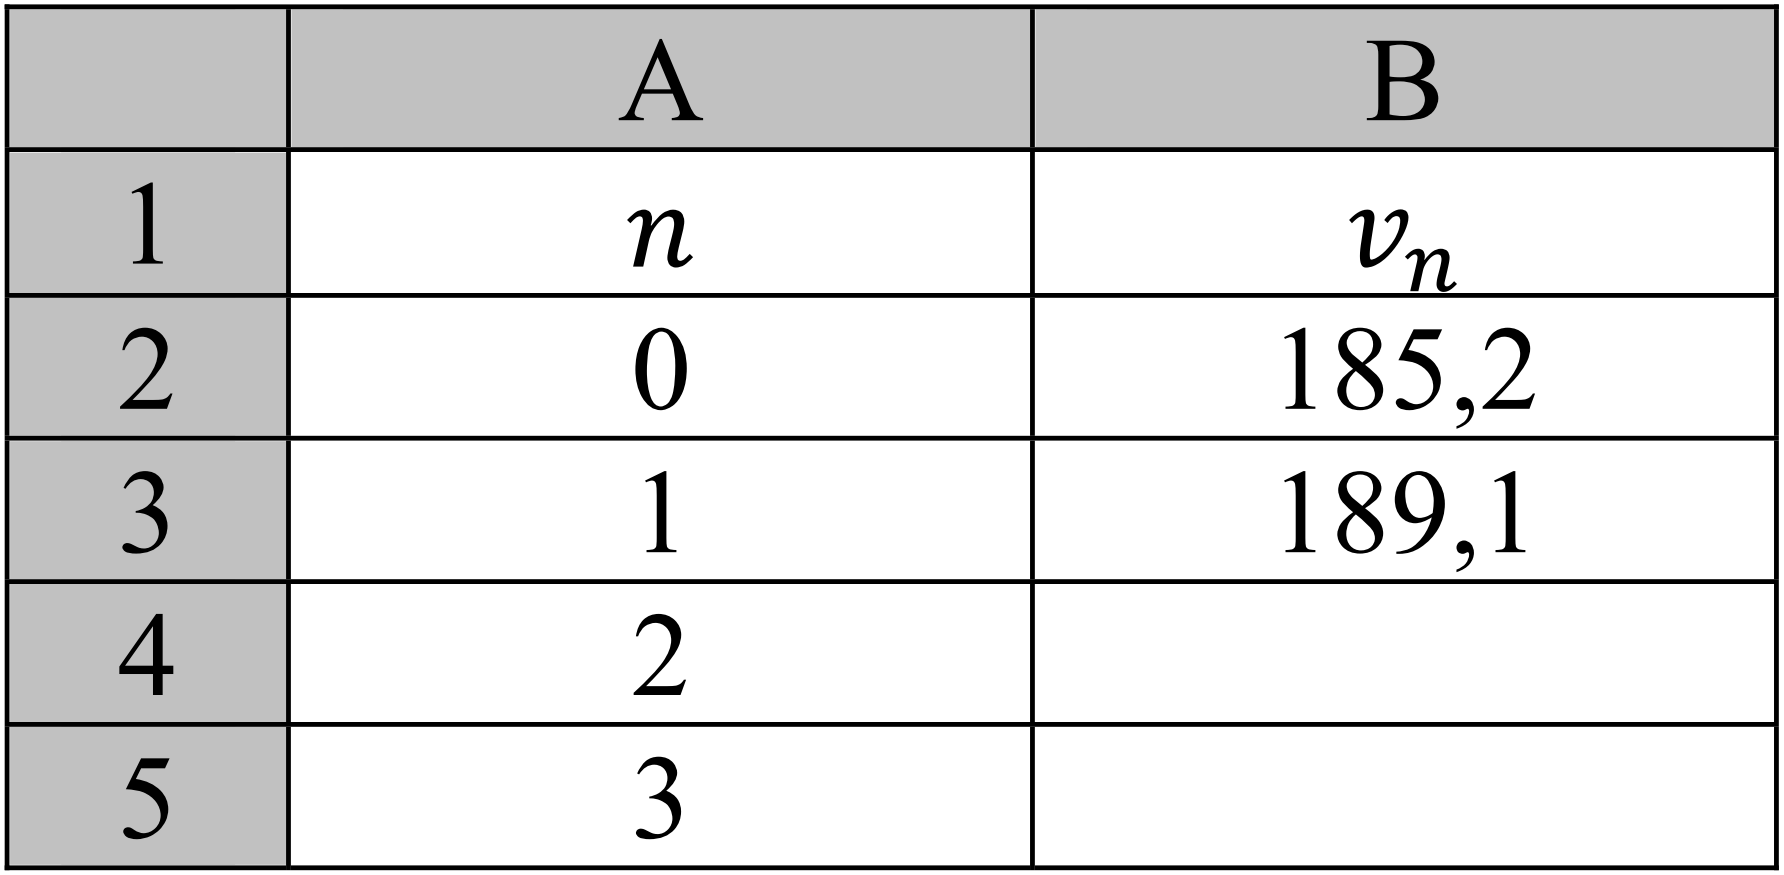
\includegraphics[scale=0.2]{img/secu}
 \end{center}

\begin{questions}
	\setcounter{question}{1}
	\question Quelle formule peut-on entrer dans la cellule $B3$, de sorte que, recopiée vers le bas, elle permette d'afficher les valeurs de la suite $(v_n)$ ?
	
	\begin{solution}
		Pour calculer les valeurs de la suite $(v_n)$, on rentre en $B4$ la formule suivante : 
		
		\begin{equation*}
			= B3 * \num{1.021}
		\end{equation*}
	\end{solution}

	\question Indiquer sans justification la nature de la suite $(v_n)$. Donner sa raison.
	
	\begin{solution}
		$(v_n)$ est une suite géométrique de raison \num{1.021}.
	\end{solution}
	
	\question Exprimer $v_n$ en fonction de $n$.
	\begin{solution}
		On a : 
		
		\begin{eqnarray*}
			v_n &=& v_0 \times q^n \\
			v_n &=& \num{185.2} \times \num{1.021}^n \\
		\end{eqnarray*}
	\end{solution}
	
	\question Déterminer une estimation de montant des dépenses d'assurance maladie voté par le parlement l'année 2020. \emph{(Arrondir la valeur à la centaine de millions.)}
	\begin{solution}
		L'année 2020 est l'année de rang 4 (2016 + 4), je calcule $v_4$ :
		
		\begin{eqnarray*}
			v_4 &=& \num{185.2} \times \num{1.021}^4 \\
			v_4 & \approx & \num{201.4}
		\end{eqnarray*}
		
		Avec ce modèle, on peut estimer le montant des dépenses d'assurance maladie voté par le parlement l'année 2020 à \num{201.4} milliards d'euros.
	\end{solution}
	
	\question \`A l'aide de la calculatrice, trouver la valeur de $x$ telle que $\num{185.2} \times \num{1.021}^x \ge \num{210}$.
	
	\begin{solution}
		\`A l'aide de la calculatrice j'obtiens $v_6 \approx \num{2019.8}$ et $v_7 \approx \num{214.2}$. On a donc $\num{185.2} \times \num{1.021}^x \ge \num{210}$ pour $x \ge 7$. 
	\end{solution}
	
	\question Déterminer, suivant ce modèle, l'année pour laquelle sera voté, pour la première fois, un montant de dépenses de l'assurance maladie supérieur à 210 milliards d'euros. 
	
	\begin{solution}
		Selon ce modèle, un montant de dépenses de l'assurance maladie supérieur à 210 milliards d'euros, sera voté pour la première fois en 2023 (2016 + 7).
	\end{solution}
\end{questions}

\section{Un QCM (6 points)}

\textit{Cet exercice se présente sous la forme d'un questionnaire à choix multiple (QCM). Pour chaque question, trois réponses sont proposées. Une seule réponses est correcte. On demande de choisir celle que vous pensez être correcte.
}


On donne le tableau de variation d'une fonction $f$ définie et dérivable sur l'intervalle $[-12, 20]$ :

\begin{center}

	\begin{tikzpicture}[scale=0.8]
		\tkzTabInit{$x$/1.5,$f'(x)$/1.5,$f(x)$/4}{$-12$, $-5$, $7$, $20$}
		\tkzTabLine { ,- ,z , +, z, -}
		\tkzTabVar{+/$7$,-/$-4$,+/$-1$,-/$-6$}
	\end{tikzpicture}

\end{center}

\begin{questions}
	\question[1] On peut dire que :
	
		\begin{checkboxes}
			\choice $f$ est positive sur l'intervalle $[-12; -5]$.
			\choice $f$ est positive sur l'intervalle $[7; 20]$.
			\correctchoice $f$ est négative sur l'intervalle $[-5; 20]$.
		\end{checkboxes}
	
		
	\question[1] L'équation $f(x)=2$ possède 
	
	\begin{oneparcheckboxes}
		
		\correctchoice une seule solution ;
		\choice aucune solution ; 
		\choice on ne peut pas répondre.
	\end{oneparcheckboxes}	

	\question[1] On cherche à comparer $f'(0)$ et $f'(8)$ :

\begin{oneparcheckboxes}
	
	
	\choice $f'(0) < f'(8)$
	\correctchoice $f'(0) > f'(8)$
	\choice on ne peut pas répondre.
\end{oneparcheckboxes}

	\question[1] On cherche à comparer $f(0)$ et $f(8)$ :
	
	\begin{oneparcheckboxes}
		
		
		\choice $f(0) < f(8)$
		\choice $f(0) > f(8)$
		\correctchoice on ne peut pas répondre.
	\end{oneparcheckboxes}



	\question[1] Une équation de la tangente à la courbe représentative de la fonction $f$ au point d'abscisse 20 est :
	
	\begin{oneparcheckboxes}
		
		
		\choice $y = 20x - 6$
		\choice $y = -x - 6$
		\correctchoice $y = -x + 14$
	\end{oneparcheckboxes}

	\question[1] On désigne par $\mathcal{C}$ la courbe représentative de $f$ dans un repère orthogonal.
	
	\begin{oneparcheckboxes}
		
		\choice Il n'existe aucun point où la tangente à la courbe $\mathcal{C}$ est parallèle à l'axe des abscisses.
		\choice Il existe un seul point où la tangente à la courbe $\mathcal{C}$ est parallèle à l'axe des abscisses.
		\correctchoice Il existe deux points où la tangente à la courbe $\mathcal{C}$ est parallèle à l'axe des abscisses.
	\end{oneparcheckboxes}	
\end{questions}





\section{(8 points)}\label{ex:apa}

L'Allocation Personnalisée à l'Autonomie en établissement (APA en établissement) est une allocation destinée aux personnes âgées de plus de 60 ans en perte d'autonomie et résidant dans un établissement de santé.


Dans cet exercice, on modélise de deux façons différentes l'évolution du montant de l'APA en établissement dans un département français.

\subsection{}

Le tableau suivant donne les montants en euro de l'APA en établissement de 2007 à 2015 pour le département considéré :

\begin{table}[h!]
	{\small \begin{tabular}{|@{\ }c@{\ }|@{\ }c@{\ }|@{\ }c@{\ }|@{\ }c@{\ }|@{\ }c@{\ }|@{\ }c@{\ }|@{\ }c@{\ }|@{\ }c@{\ }|@{\ }c@{\ }|@{\ }c@{\ }|}
	\hline
	Année                   & 2007        & 2008        & 2009        & 2010        & 2011        & 2012        & 2013        & 2014        & 2015        \\ \hline
	Rang de l'année ($x_i$) & 1           & 2           & 3           & 4           & 5           & 6           & 7           & 8           & 9           \\ \hline
	Montant, en euro de     &             &             &             &             &             &             &             &             &             \\ 
	l'APA en établissement  & \num{13504} & \num{14443} & \num{14914} & \num{15351} & \num{15751} & \num{16144} & \num{16744} & \num{17190} & \num{18070} \\ 
	($y_i$)                 &             &             &             &             &             &             &             &             &             \\ \hline
\end{tabular}}

\end{table}
En annexe \ref{sec:nuage}, à rendre avec la copie, on a représenté, dans un repère orthogonal, le nuage de points de coordonnées $(x_i ; y_i)$ associé à cette série statistique.

\begin{questions}
	
	\question
	\begin{parts}
		\part Déterminer les coordonnées du point moyen $G$ de ce nuage de points. Arrondir l'ordonnée à l'unité.
		\begin{solution}
			
			\begin{equation*}
			\bar{x} = \dfrac{1 + 2 + 3 + 4 + 5 + 6 + 7 + 8 + 9}{9} = 5
			\end{equation*}
			
			
			\begin{footnotesize}
				\begin{equation*}
				\bar{y} = \dfrac{\num{13504} + \num{14443} + \num{14914} + \num{15351} + \num{15751} + \num{16144} + \num{16744} + \num{17190} + \num{18070}}{9} \approx \num{15790.1}
			\end{equation*}
			\end{footnotesize}
			
			Le point moyen du nuage est $G(5 ; \num{15790})$.
		\end{solution}
	
		\part Placer le point $G$ dans le repère précédent.
	\end{parts}

	\question On admet que la droite $D$ d'équation $y=\num{516}x + \num{13210} $ réalise un bon ajustement affine du nuage de points jusqu'en 2020.
	
		\begin{parts}
			\part Tracer la droite $D$ dans le repère précédent. Donner les coordonnées des points choisis pour la tracer.
			
			\begin{solution}
				Soit A, le point de la droite $D$, d'abscisse 0, on a $A(0 ; y_A) $.
				
				\begin{eqnarray*}
					y_A &=& 516 \times x_A + \num{13210} \\
					y_A &=& 516 \times 0 + \num{13210} \\
					y_A &=& \num{13210} \\
				\end{eqnarray*}
			
				Pour tracer la droite $D$, j'utilise donc les points $A(0;\num{13210})$ et $G(5 ; \num{15790})$.
				
				\begin{center}
					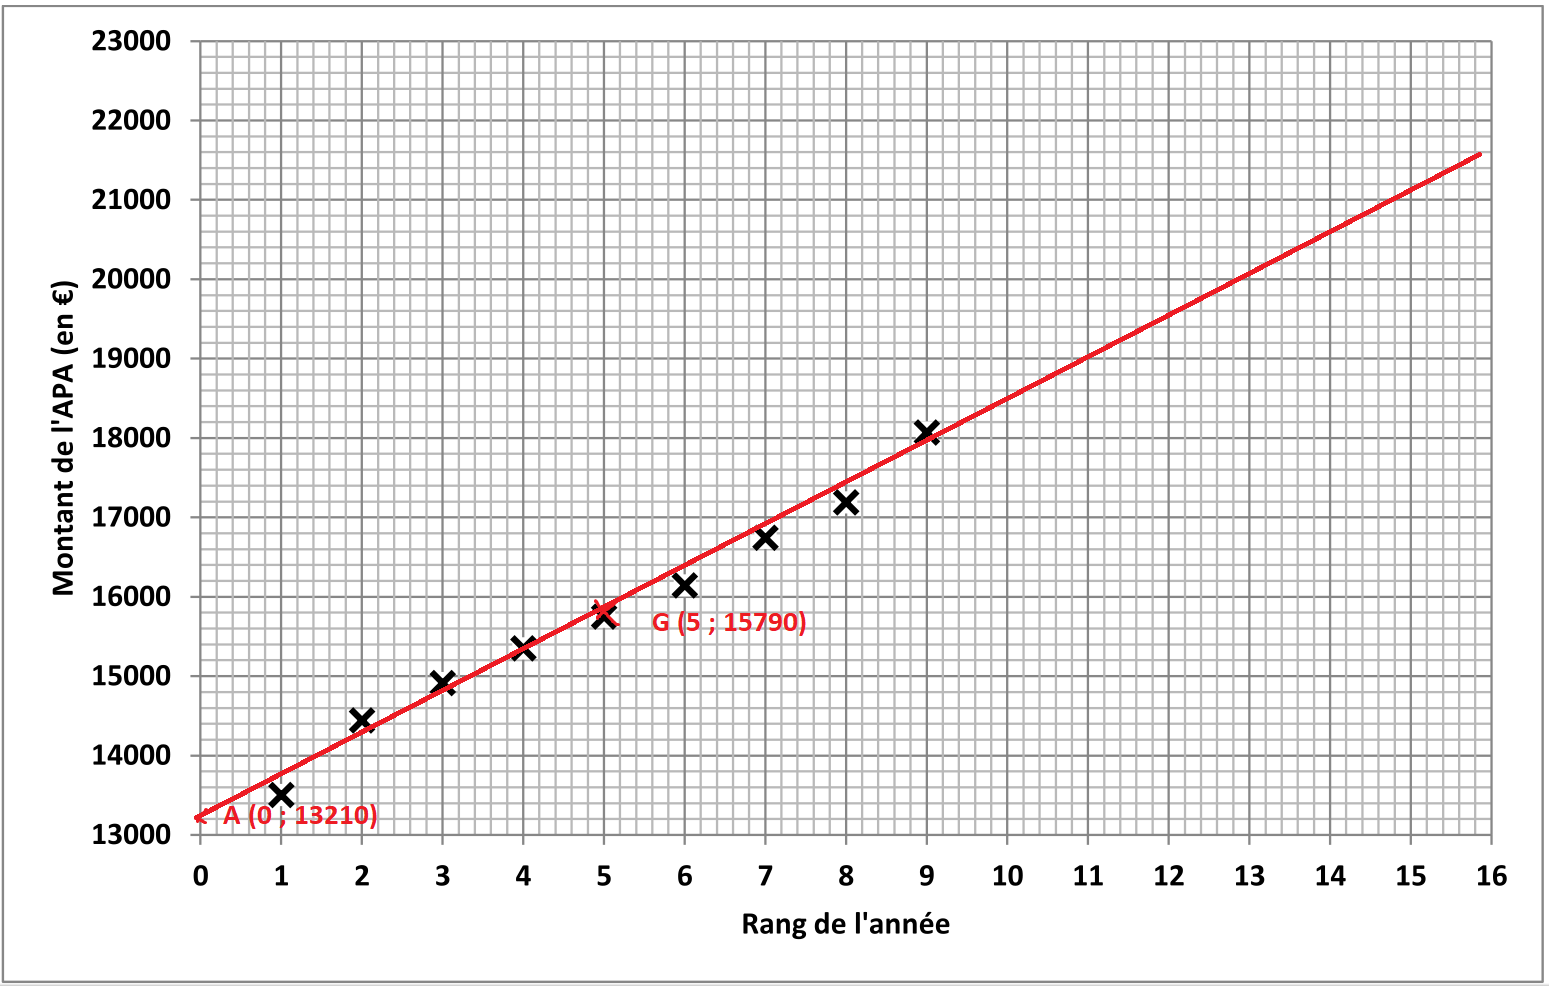
\includegraphics[scale=0.35]{img/graph_corr}
				\end{center}
			\end{solution}
			
			\part \`A l'aide de cet ajustement, donner une estimation du montant de l'APA en établissement dans ce département pour l'année 2018.
			
			\begin{solution}
				2018 est l'année de rang 12. Dans l'équation de la droite, je remplace donc $x$ par 12.
				
				\begin{eqnarray*}
					y &=& 516 \times 12 + \num{13210} \\
					y &=& \num{19402} \\
				\end{eqnarray*}
			
				On peut donc estimer que le montant de l'APA en établissement dans ce département en 2018 sera de \num{19402} €.
			\end{solution}
		\end{parts}
\end{questions}

%\newpage
\subsection{}

On a recopié le tableau précédent dans une feuille de calcul d'un tableur.
Les cellules de la ligne 4 sont au format pourcentage.

\begin{center}
	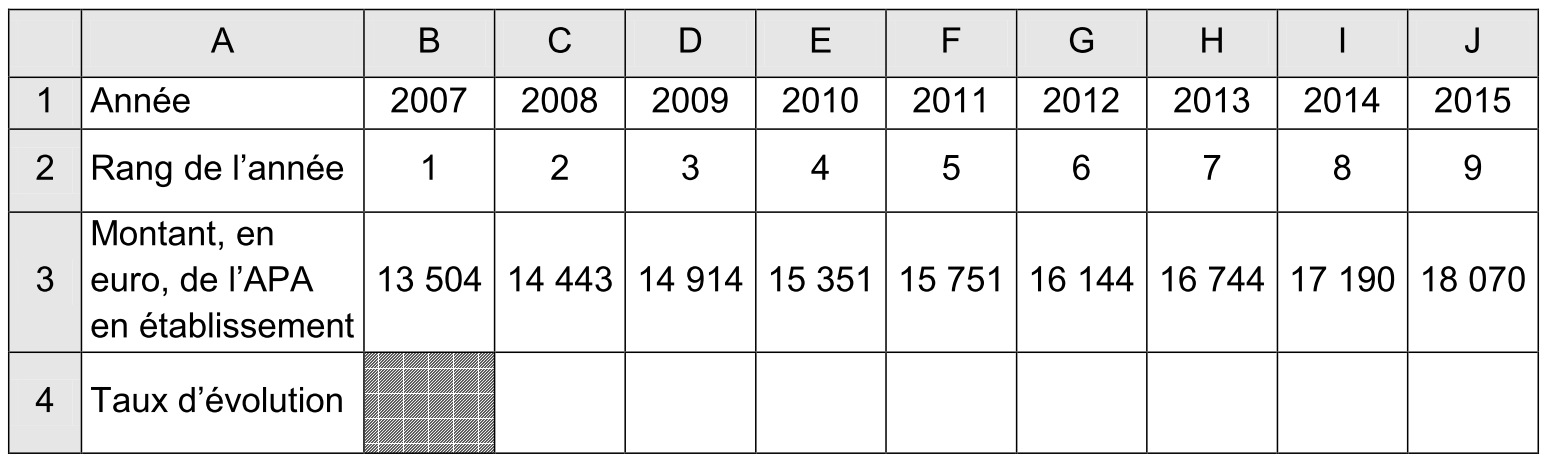
\includegraphics[scale=0.4]{img/tab_apa}
\end{center}


\begin{questions}
	\question 
		\begin{parts}
			\part Calculer le taux d'évolution de montant de l'APA en établissement dans ce département entre 2014 et 2015. Arrondir le résultat à \num{0.1} \%.
			\begin{solution}
				\begin{eqnarray*}
					t &=& \dfrac{v_{arrivée} - v_{départ}}{v_{départ}} \\
					t &=& \dfrac{\num{18070} - \num{17190}}{\num{17190}} \\
					t &\approx&  \num{0.051}
				\end{eqnarray*}
				
				Entre 2014 et 2015; l'APA en établissement a augmenté de \num{5.1} \% dans ce département.
			\end{solution}
			
			\part Quelle formule doit-on entrer dans la case $C4$ pour obtenir, par recopié vers la droite, les taux d'évolution en pourcentage du montant de l'APA en établissement dans ce département, entre deux années consécutives ?
			
			\begin{solution}
				Pour calculer le taux d'évolution on rentre en $C4$ la formule suivante : \\ $=(C3 - B3)/B3$.				
			\end{solution}
		\end{parts}
	
	
	\question On suppose maintenant que le montant de l'APA en établissement dans ce département augmente de \num{5.1} \% par an après 2015. On décide de modéliser ce montant par une suite numérique $(u_n)$.
	
	
		
	Pour tout entier naturel $n$; $u_n$ désigne le montant de l'APA en établissement dans ce département, en euro, pour l'année $(2015 + n)$. Ainsi $u_0 = \num{18070}$.
		\begin{parts}
			\part Calculer $u_1$. Arrondir le résultat à l'unité. Interpréter la valeur de $u_1$ dans le contexte de l'exercice.
			\begin{solution}
				L'APA en établissement augmente chaque année de \num{5.1} \%, donc pour passer d'une année à l'autre, on multiplie le montant par \num{1.051}. On a donc :
					
					\begin{eqnarray*}
						u_1 &=& u_0 \times \num{1.051} \\
						u_1 &=& \num{18070} \times \num{1.051} \\
						u_1 &\approx& \num{18991.6} \\
					\end{eqnarray*}
					
					$u_1$ représente le montant de l'APA en établissement dans ce département en 2016.
				\end{solution}
				
			\part Donner, sans justification, la nature de la suite $(u_n)$ et sa raison.
			\begin{solution}
				$(u_n)$ est une suite géométrique de raison \num{1.051}.
			\end{solution}
				
			\part Exprimer, pour tout entier naturel n, $u_n$ en fonction de $n$.
			\begin{solution}
				On a : 
				
				\begin{eqnarray*}
					u_n &=& u_0 \times q^n \\
					u_n &=& \num{18070} \times \num{1.051}^n \\
				\end{eqnarray*}
			\end{solution}
		\end{parts}
	
	\question Parmi les deux modèles (l'ajustement affine de la partie A et la suite $(u_n)$ de la partie B), quel est celui qui prévoit le plus haut montant de l'APA en établissement pour l'année 2018 ?
	
	\begin{solution}
		L'année 2018 est l'année de rang 3 (2015 + 3), je calcule $u_3$ :
		
		\begin{eqnarray*}
			u_3 &=& \num{18070} \times \num{1.051}^3 \\
			u_3 & \approx & \num{20978}
		\end{eqnarray*}
	
		\num{20978} > \num{19402}, c'est donc la suite $(u_n)$ qui prévoit le plus haut montant de l'APA en établissement en 2018.
	\end{solution}
\end{questions}

\newpage

\appendix

\titleformat{\section}{\Large\bfseries}{\appendixname~\thesection .}{0.5em}{}
\section{}\label{sec:nuage}


\begin{center}
	 {\Large \'A rendre avec la copie
	 
	 \ref{ex:apa}}
 
 	\vspace*{1cm}
	
	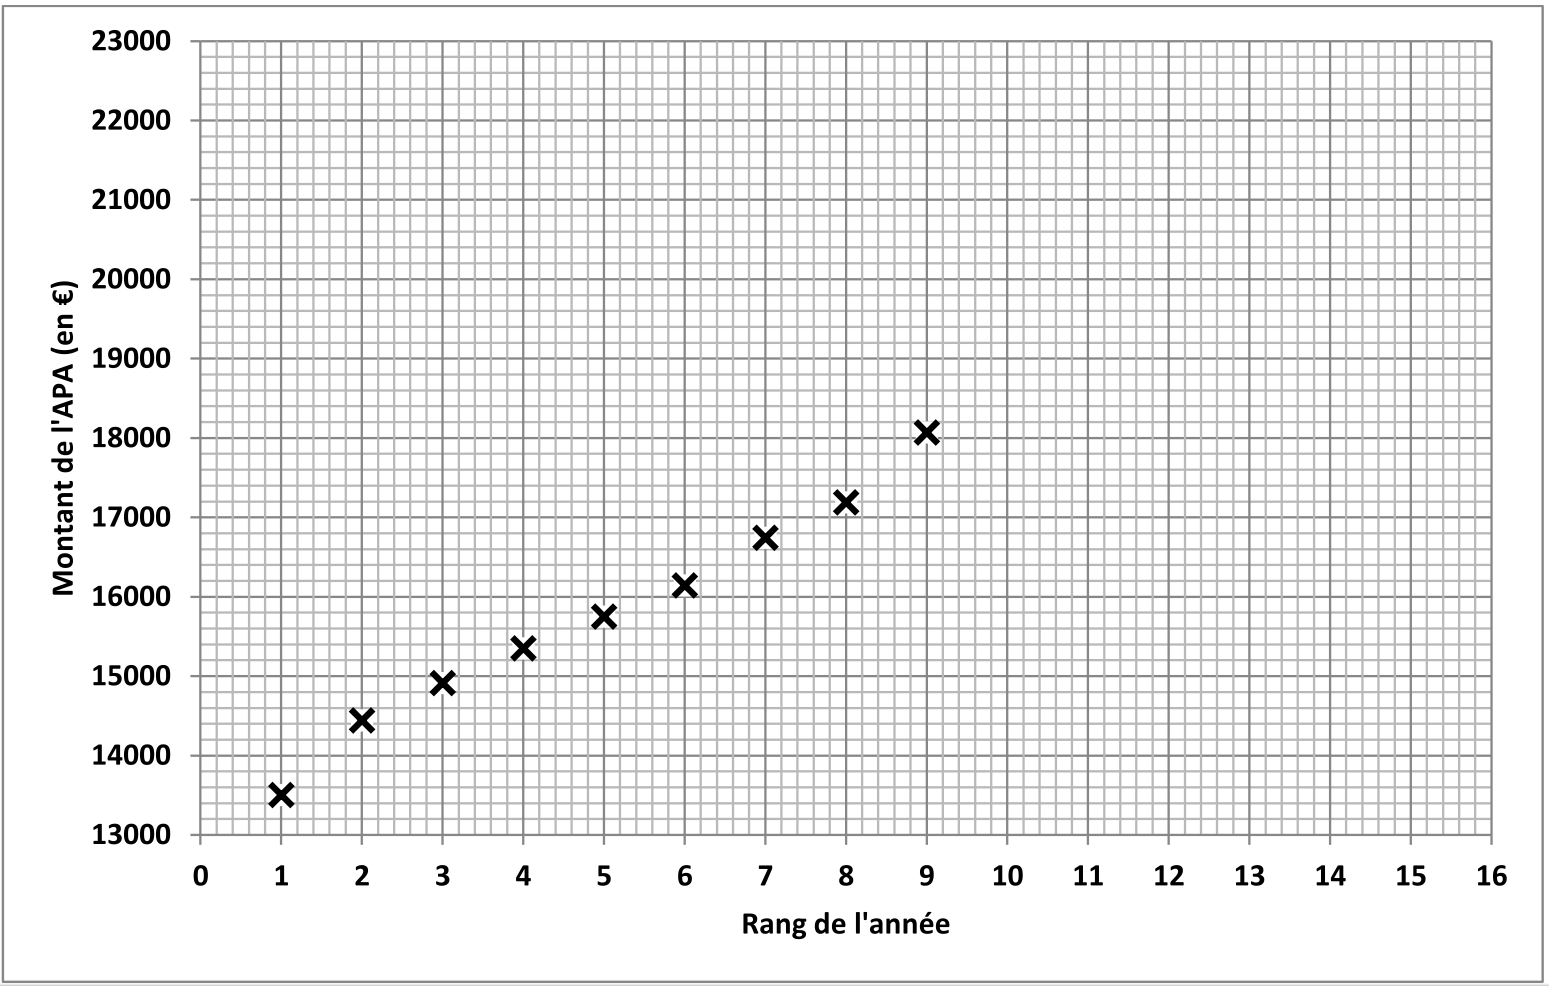
\includegraphics[scale=0.43]{img/graph}
	

\end{center}

\label{annexe}
	\label{LastPage}
	

\end{document}